\chapter{绪\hskip 0.4cm 论}
\label{chap1}

\section{研究背景及意义}
随着信息时代的发展,信息安全,网络安全,系统安全在社会中的作用日益重要起来。互联网作为一个自由开放,虚拟交互的全球平台,可以使人们更便利的获取,发布信息,但与此同时,互联网与个人息息相关的的资源也受到不同程度的威胁,于是安全技术研究也蓬勃发展起来。传统计算机的出现,使得古典密码的破解变得容易,计算机网络的数据传输需要更安全的密码算法,于是产生了一些经典的加密算法,如:DES,AES等对称加密算法,RSA,ECC(椭圆曲线加密算法)等非对称加密算法。密码设计者与密码分析者相互竞技,共同促进密码学平衡的发展。但是,量子计算机的问世,让密码学领域的格局发生了巨大的变化。

\begin{figure}[H]
	\centering
	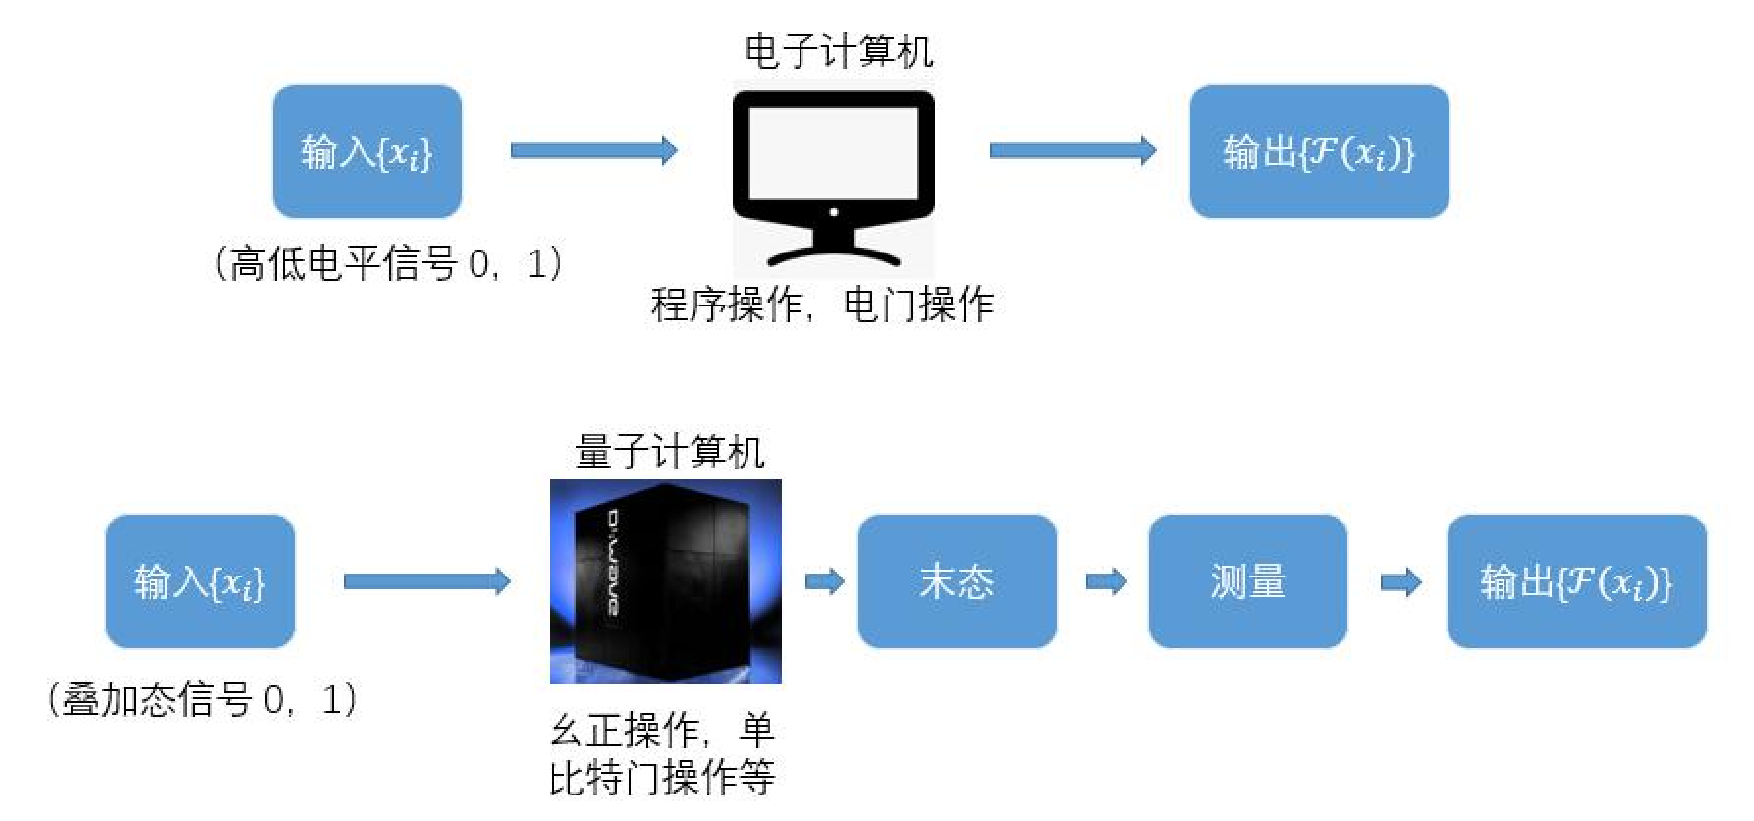
\includegraphics[width=15 cm]{fig/quantum.pdf}
	\caption{量子计算机与普通计算机的区别} %\vspace*{-1.0cm}
	\label{fig:quantum_pdf}
\end{figure}

密码学技术,是安全技术研究的基石,其实从古至今都不乏密码学的研究,自密码学从外交情报和军事领域走向公开后,社会信息流通的方式,也深刻影响着密码学的特点。量子计算机作为第六类计算机,使用的计算方式和平常使用的普通计算机非常不同,如图\ref{fig:quantum_pdf}。量子计算机使用量子位进行计算,可以将普通计算机需要执行几十年的任务在几秒钟之内完成。目前出现的一些量子算法,如 Shor 算法\cite{Shor1994Algorithms}和 Grover 算法\cite{Grover1996Fast}已经对互联网中应用广泛的 RSA 算法、ElGamal算法、ECC公钥密码算法和Diffie-Hellamn密钥协商协议进行有效的密码攻击。如此以来,经典加密算法将受到严重的威胁,虽然在短时间内量子计算机的硬件成本和理论模型实际运作的难度不会让量子计算机真正的破解已经在商用的密码算法,但是为了防范未来量子计算机的攻击,许多种防御量子计算的加密算法也在研究之中。比如:基于Hash函数的公钥密码体制、基于格问题的公钥密码体制、基于多变量问题的公钥密码体制、基于编码问题的公钥密码体制。本文主要讨论的是基于编码问题的公钥密码体制。作为抵御量子计算机攻击的算法,基于编码的加密算法的理论基础却不是来源于量子物理,它的理论来源是信息论,编码理论,代数理论等数学知识。

基于编码的加密算法,就不会受到Shor算法或者Grover算法的影响,从而保证网络通信的安全。50年代,随着C.E Shanon《通信的数学理论》的发表,信道编码定理给出了提高多类信道上传输消息的效率,采用性质良好的纠错码的指导。60年代纠错码的研究进入快速发展期,期间有广泛应用的汉明码、Reed-Muller码、BCH码、Goppa码等等。纠错码具备的检查错误或纠正错误的能力,被很好的应用到了公钥密码体制中。1978年,McEliece首次提出基于编码的公钥加密方案,采用可以快速译码的Goppa码,安全性依赖于一般线性码译码问题(NP-完全问题)。在一些已知的攻击算法中,其工作因子都是在$2 ^ {70}$以上,具备较高的安全性。其变形方案Niderreiter公钥密码体制在公钥私钥设置中有所不同,但在安全性上被证明是等价的。

在之后的研究中,基于编码的加密方案在码的选择和公钥的构造方式上做了很多尝试,目的就是为了减小公钥大小和提升算法效率,使得在实际中快速落地,获得更好的发展,以做好应对几年之后量子攻击的准备。综上所述,研究基于编码的加密方案具有十分重要的意义。

\section{国内外研究现状}
公钥密码技术经历近五十年的发展,已经被广泛的应用到计算机系统领域,互联网通信领域中。工业界应用公钥加密的案例数不胜数。网络安全访问的实现就是集成了 RSA 的加密与解密功能,极大的解决了网络中的密钥分发与密钥管理的问题。相对于对称密码在数字签名领域的局限性,公钥密码技术可以很好的实现唯一性,私有性等数字签名的要求,通过私钥签名由对应的公钥去验证,其他人无法冒名顶替,无法篡改签名内容,从而提供网络中的数字签名服务。在身份鉴别领域,通过公钥密码技术实现的方案在执行起来也比对称密码简单得多。公钥密码技术的安全性,基于两大数论难题:\ding{172} 大整数分解的难解性问题,\ding{173} 离散对数问题的难解性。后续在经典数论的基础上,RSA,ECC,Rabin等算法都在不断的改进中,以适应越来越有挑战的密码攻击。但是随着 Shor,Grover 等量子算法针对性的出现,建立在经典数论的公钥密码技术处于集体沦陷的趋势,此时抗量子密码体制逐渐成为公钥密码研究的方向之一,目的就是为了防范量子计算机算法带来的安全威胁。

基于编码的加密算法,之所以能够抵御量子计算机的攻击,是因为量子攻击算法只能攻破上述两大难题,而攻不破{NP-}完全问题。McEliece在1978年首次提出基于编码的加密方案,它的安全性假设是二元随机码的译码问题\cite{Berlekamp1978On}以及Goppa码的随机码的区分问题\cite{Engelbert2007A},这两个问题在相关专家学者的研究中被证明是{NP-}完全问题,原始的McEliece方案经过三十多年的密码分析,被认为是目前为止最安全的公钥密码方案之一。McEliece方案采用一个随机二元不可约Goppa码作为私钥,也就是说保密Goppa码的生成矩阵,公钥是对生成矩阵进行混淆和交换后公开的随机生成矩阵。加密过程中,就是将明文加密成合法码字,并加入尽可能多可纠错的差错向量发送给消息接收者。消息接收者就可以使用私钥,消除密文中冗余的错误信息,从而正确译码。相对于RSA,McEliece方案因为Goppa码拥有快速译码的算法,在加解密的运算中都有高效的优势。但是公钥尺寸过大的问题,一直是McEliece方案无法真正取代经典公钥密码算法的主要原因之一。

Niderreiter方案\cite{Niederreiter1986Knapsack}是McEliece方案的一种对偶变形,如图 \ref{fig:comparator_pdf},是一种背包型的密码体制。与McEliece方案不同,Niederreiter方案首先运用函数将消息编码成一个错误向量,用错误向量代表消息,私钥同样是一个随机GRS码,公钥是码的校验矩阵混淆和交换后的矩阵,加密过程是计算公钥矩阵和错误向量一个伴随式,解密的时候利用GRS码的伴随式译码算法,恢复明文消息。Niderreiter方案与McEliece方案的安全性是等价的,设计Niderreiter的初衷是为了缩小公钥的规模,在存储公钥的时候只需要存储公钥的冗余部分。但是在将明文映射到差错向量时,加解密的速度较慢。

\begin{figure}[H]
	\centering
	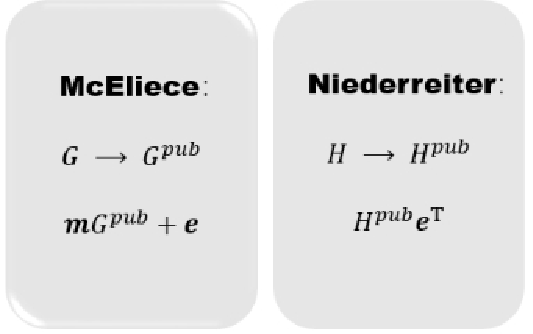
\includegraphics{fig/comparator.pdf}
	\caption{方案公钥,加密过程对比} %\vspace*{-1.0cm}
	\label{fig:comparator_pdf}
\end{figure}

后续的研究中,相关专家学者在码的选择上做了充分的分析。因为GRS码密钥的紧凑性,基于GRS码的加密方案一经提出就被认为是比Goppa码更适合的方案。但根据\cite{Couvreur2013Distinguisher}的密码分析结果,基于GRS 码的加密方案已经是不够安全的。在\cite{Loidreau2017A}中,Gabidulin编码也已经应用到McEliece加密方案中,Gabidulin码在度量的选择上与其它方案不同,前者是基于秩度量,后者都是基于汉明度量。实际上因为Gabidulin码在Frobenius自同构下包含巨大的向量空间不变性导致结构上的弱点明显,基于秩度量的方案在安全性上也不可靠。1994年,SideInikov在他的研究中使用Reed-Muller码字构造了公钥加密算法\cite{Sidel1994Open},该算法具有非常高效的解码算法。后续还有很多其它的基于编码的密码方案。到目前为止,安全参数下的McEliece方案仍未被打破。另外,在\cite{Courtois2001How}中提出了 McEliece(或 Niderreiter)方案的数字签名方案。在\cite{Baldi2007Cryptanalysis}中,低密度奇偶校验码LDPC表示前向纠错技术,并允许接近香农理论极限的现有好性质的码。它可以减小密钥大小,提高传输效率。但是在\cite{Baldi2008A}的分析中,它所特有的稀疏公钥矩阵可能会暴露私有代码结构属性。目前,有人建议使用中等密度奇偶校验码MDPC来设计公钥密码系统\cite{Misoczki2013MDPC},希望在所提出方案的密钥安全性和公钥大小之间找到良好的平衡。尽管这些基于编码的加密或签名方案没有被完全攻破,但是这些方案因为安全参数下公钥尺寸过大,所以并不适应作为标准的加密程序。因此,我们迫切需要设计基于编码的紧凑公钥和私钥结构混淆良好的加密方案。

\section{本文工作与主要贡献}
2016年,Baldi等人提出了McEliece密码系统的新变体(简称BBCRS方案)。其中,McEliece中置换矩阵$P$由低秩矩阵$R$和广义置换矩阵$T$构造的矩阵$Q$替代。这使得BBCRS方案能够实现私钥不再与公钥存在置换相等的特性,从而允许在BBCRS方案中采用一些高性能的码,例如GRS码来减小公钥大小。不幸的是,Baldi等人提出的方案的生成密钥的两个案例都是不安全的。另一方面,我们注意到解密过程中需要猜测满足条件的向量以消除在解密过程期间添加的差错向量的影响,这将会是很大的工作量,尤其是当有限域的元素很多,也就是$q$值比较大的情况。

受BBCRS方案的影响,我们提出了一种新的公钥生成方法,避免了BBCRS方案在解密过程中需要的大量试错操作。此外,我们的新方案中的解密方式能够最大化码字的纠错能力来处理所接收的密文,从而增加消息的传输率。因此,我们可以考虑减小消息长度以获得适当大小的密钥。 此外,我们提出了构造矩阵$R$的新方式,其在效率和存储方面与构建在BBCRS方案中建议的第一种情况相当。这种新方式的主要优点是它可以更好地隐藏密钥结构。这使得在不降低安全级别的情况下,能够在方案中采用强结构的码族。

\section{研究重点与组织结构}
第一章为绪论,主要介绍了抗量子密码的研究背景及意义,也讨论了国内外的研究现状,接着对文章的主要工作做了基本概括,最后对文章的章节做了介绍。

第二章是预备知识与概念的梳理,包括编码理论基础知识、解码算法、常见的码的性质的简要介绍。

第三章主要是对经典的基于编码的加密方案,进行系统概述。第四章着重介绍本文实现的改进方案,原理及分析等。

第五章讨论了解码算法对加密方案的影响。

第六章总结全文内容,并展望未来研究工作的方向。